\documentclass[preprint,10pt,oneside,onecolumn,authoryear]{elsarticle}
\journal{Journal of Archaeological Science: Reports}

\usepackage[utf8]{inputenc}
\usepackage[T1]{fontenc}
\usepackage{amsmath}
\usepackage{amsfonts}
\usepackage{amssymb}
\usepackage{graphicx}
\usepackage{subcaption}
\usepackage[english]{babel}
\usepackage{natbib}
%\bibliographystyle{abbrvnat}
\usepackage{lineno}
\usepackage{float}
\usepackage[hidelinks]{hyperref}

\begin{document}
\linenumbers

\begin{frontmatter}

\title{On and Off the Rivers: Changes in Clay Sourcing and Preparation Strategies in the Congo Basin throughout the past two Millennia}
%\subtitle{Strategies for Clay Sourcing and Preparation in Central Africa}
\author[1]{Dirk Seidensticker\corref{cor1}}
\ead{dirk.seidensticker@ugent.be}

\author[2]{Wannes Hubau}

\author[3]{Florias Mees}

\author[4,5]{Géraldine Fiers}

\author[4]{Veerle Cnudde}

\cortext[cor1]{Corresponding author}
	
\affiliation[1]{organization={Ghent University, Department of Archaeology}, 
	addressline={Sint-Pietersnieuwstraat 35},
	postcode={9000},
	city={Ghent},
	country={Belgium}}

\affiliation[2]{organization={Ghent University, Department of Environment}, 
	addressline={Coupure links 653},
	postcode={9000},
	city={Ghent},
	country={Belgium}}

\affiliation[3]{organization={Royal Museum for Central Africa, Department of Earth Sciences}, 
	addressline={Leuvensesteenweg 13},
	postcode={3080},
	city={Tervuren},
	country={Belgium}}

\affiliation[4]{organization={Ghent University, Department of Geology}, 
	addressline={Krijgslaan 281},
	postcode={9000},
	city={Ghent},
	country={Belgium}}

\affiliation[5]{organization={Utrecht University, Department of Earth Sciences}, 
	addressline={Princetonlaan 8a},
	postcode={3584},
	city={Utrecht},
	country={The Netherlands}}

\begin{abstract}
Pottery constitute the most prominent find category encountered by archaeologists in Central Africa and is utilized as basis for various regional chrono-historical typologies. The resulting sequences of inter-related pottery styles are often regarded as proxies for the transfer of knowledge within potters' genealogies of practice, despite little being known about the technical approaches ancient potters' communities followed. This paper presents, for the first time, petrographic and geochemical data to deduce, not only the 'local, intermediate or trans-local nature' of vessel units, but more importantly clay sourcing and preparation strategies of potters' communities throughout the past two millennia. A unique fieldwork strategy, specifically river-bound surveys along the main tributaries of the Congo River, shaped the archaeological record of the Congo Basin considerably. The results from the two case studies selected for this analysis inform on distinct strategies for clay sourcing, most importantly the exclusive reliance of potters either of fluvial clays that were used without tempering and occasionally tempered clays of unknown provenance. The former type is only superficially known in sub-Saharan Africa as of jet. This study also incorporated finds made some distance away from the rivers, on the \textit{terra firme}, that show unique characteristics when compared to inventories from nearby sites close to the rivers. These finds, made during paleo-environmental research, are informative over the potential biases earlier river-bound research had.
\end{abstract}

\begin{keyword}
Congo Basin \sep Pottery \sep Petrography \sep Handheld XRF \sep Clay Sourcing
\end{keyword}

\end{frontmatter}

\newpage

\section{Introduction}

Ceramics are the main aspect of material culture archaeological research uncovered in the Congo Basin. The stylistic evolution and subsequently deduced reconstructions of settlement processes showed diverse regional lines of development. While the continues sequences of pottery styles in the Inner Congo Basin indicate some permanence of communities \citep{Wotzka.1995}, research in the northern and western \citep{Seidensticker.2021e,Seidensticker.2024} as well as the north-eastern parts of the basin \citep{LivingstoneSmith.2017} point at disruptions of established communities \citep{Seidensticker.2021,Seidensticker.2021e,Seidensticker.2025}. Most studies focused on formal attributes, such as vessel shapes and decorations, to conceptualize pottery styles. This means that little is known about the technical approaches ancient potters' communities followed. They facilitate the reconstruction of production sequences or \textit{chaînes opératoires} and are vital to gain deeper insight into the social cohesion within communities producing pottery of a similar style and their change through time.

Knowledge relating to the initial stages of the \textit{chaînes opératoires} of potters' genealogies of practice \citep{Gosselain.2018} in the Congo Basin, dating back to the onset of pottery production in the 4th to 2nd century BCE \citep{Wotzka.1995}, are very rare. While some insight might be drawn from neighboring regions \citep{Mercader.2000,Tsoupra.2022,EpossiNtah.2024}, most information on raw material procurement and preparation stems from ethnographic observations \citep{Coart.1907,Maes.1937,Eggert.1980c,KanimbaMisago.1992a}. The prevailing hypothesis is that secondary clays originating in rivers, streams, lakes or swamps are the main source for potters in the Congo Basin \citep[18--19 Map~1]{Drost.1967}. \citet[31--32]{Coart.1907} conclude that the vast river networks of the Congo Basin offer easy accessibility to fluvial clays, such as Kaolin. Only in the south-western Congo Basin, near Lake Mai-Ndombe, records indicate that clays originating from termite mounts were used as well \citep[19--21 Map 1]{Drost.1967}.
 
 \begin{figure*}[p]
 	\centering
 	\includegraphics[height=.85\textheight]{Fig_Map_Top.jpg}
 	\caption{A) Map of the study area with studied sites (black) and sites mentioned in the text (grey). Dark shading in the insert map shows the modern distribution of the equatorial rainforest after \citet{White.1983}. B) Topographic setting of studied sites. Catchment areas are plotted at 10~km distances. Dashed circles indicate 3~km \citep[35]{Gosselain.2005} and 7~km \citep[452]{Whitbread.2001} putative catchment areas for the sourcing of clay by potters. Topography was derived of elevation data provided by \citet{Hollister.2022}. Note that the sites in the Salonga National Park are the only ones at some distance from the river, while all other sites are located on the banks of mayor rivers.}
 \label{fig:map}
\end{figure*}

\begin{figure}[!tb]
	\centering
	\includegraphics[width=.9\textwidth]{Fig_PotteryChrono.pdf}
	\caption{Temporal distribution of known pottery styles identified at Pikunda and Munda (A) as well as Monkoto and Wafanya (B). At Munda, only pottery of the styles Pikunda-Munda and Ebambe (A) was encountered. Circles represent the highest probability of calibrated calendar ages for each pottery-linked 14C date. The intensity of grey-shading is proportional to the summed probability of the calendar-age windows of all radiocarbon dates by type. Colored bars represent the phase duration of radiocarbon dates pottery styles. For groups with more than two associated radiocarbon dates, the phases’ median start and end dates were calculated using a Bayesian model \citep[Fig.~S1, Tab.~S1]{Crema.2021a,Crema.2021b,Seidensticker.2024}. Dashed colored bars indicate estimated bins derived from stylistic resemblance \citep[218--244 Fig.~100--107]{Seidensticker.2021,Seidensticker.2021e}.}
	\label{fig:chrono}
\end{figure}

A systematic description of the \textit{chaîne opératoire} of a present-day potters' community is thus far only known from the main potters' village of the Inner Congo Basin, Ikenge on the Ruki river \citep{Eggert.1980c,Wotzka.1991,KanimbaMisago.1992a}. At this village of around 250 inhabitants in the late 1970s, all of the nearly 100 adult women produced pottery to be traded at the local and regional markets as well as at passing-by larger riverboats \citep{Eggert.1991}. Clay is extracted at the Luako, a small inlet about 4.5--6~km downstream from Ikenge, north of the Ruki river \citep[389 Fig.~1]{Eggert.1980c}, which required on average a one to two hour trip with the dugout \citep[43]{KanimbaMisago.1992a}. The clays, called "yomba" \citep[33]{Engels.1912}, are either white or dark \citep[290]{Wotzka.1991} and collected in areas that are private family properties, with ownership being derived via ancestry \citep[396]{Eggert.1980c}. Unlike in other parts of the Congo \citep[33]{Coart.1907}, clay's are no trade-goods at Ikenge. Only access-rights to specific sources can be bought by potters without a family source \citep[396]{Eggert.1980c}. Extracted clays are stored submerged in the river near the village to avoid drying out, which gives the clay more binder \citep[33--34]{Coart.1907} \& \citep[29]{Maes.1937}. The clays are moisturized and kneaded by hand right before potting. During this process, coarse materials and impurities are removed \citep[397]{Eggert.1980c}. No additional non-plastic components are added during the processing stage. As the raw clays already show a good balance between plastic and non-plastic components adding temper agents is avoided to prevent shrinkage and cracking during drying and firing \citep[397]{Eggert.1980c}. At the time, it was unknown that the clays contain large quantities of sponge spicules, which make them naturally tempered. The usage of un-tempered fluvial clays, while being reported from the region \citep[35]{Coart.1907}, is regarded as exception on a supra-regional scale \citep[30-33]{Drost.1967}.

The main source of the archaeological knowledge of the Congo Basin are widespread surveys and excavations conducted by the \textit{River Reconnaissance Project} led by Manfred K. H. Eggert between 1977 and 1987 \citep{Eggert.1978,Eggert.1987d,Eggert.1983,Eggert.1984,Eggert.1984a,Eggert.1987a,Eggert.1992,Eggert.1993}. In total about 5.000~km of rivers and 307 locations, mostly modern villages, were surveyed. At 23 of these locations 80 test trenches were excavated \citep[295 Fig.~16.2]{Eggert.1993}. The results of this projects fieldwork have been studied and published in detail \citep{Wotzka.1995,Seidensticker.2021e}. 

This paper's main objective is to deduce the clay sourcing and preparation strategies of potters' communities based on novel mineralogical and geo-chemical data that were obtained from ceramics originating from archaeological, ethnographical and environmental research in two distinct regional settings, henceforth denoted as case studies I and II (Fig.~\ref{fig:map}A). The pottery inventories from both these study areas cover substantial parts of the regional as well as supra-regional sequence of pottery development \citep[Fig.~\ref{fig:chrono};][]{Wotzka.1995,Seidensticker.2021e}. A secondary objective aims at debating the issue of potential sampling biases due to the focus on river surveys during the fieldwork of the \textit{River Reconnaissance Project}, especially in light of new finds that were made on the \textit{terra firme} close to the Luilaka river.

\section{Methods and Materials}

\begin{table}[p]
	\centering
	\includegraphics[height=.88\textheight]{Tab_Samples.pdf}
	\caption{List of samples included in this study and applied methods. Type of sherds are seperated for complete or nearly complete vessels, vessel parts of which considerable parts are missing but the entire profile from the rim to the base can be reconstructed and wall fragments with either the rim or base missing. The samples were subjected to petrographic (P) and geo-chemical analysis (C).}
	\label{tab:samples}	
\end{table}

\subsection{Materials}

The study is comprised of 43 samples from five different sites (Tab.~\ref{tab:samples}) . Samples for case study I---the western Congo Basin---were taken from the inventories of the site of Pikunda along the middle Sangha river and Munda at the upper Likwala-aux-Herbes river (Fig.~\ref{fig:map}). Pikunda and Munda are the only excavated sites in this region that yielded pottery inventories from multiple chronological phases \citep{Seidensticker.2021e}. The earliest wide-spread type of ceramics found in the western Congo Basin was names after these two sites \citep[114--120]{Eggert.1992,Seidensticker.2021e}.

In total, 15 sherds from Pikunda were sampled for this study (Tab.~\ref{tab:samples}). Among these are three sherds of the Pikunda-Munda style \citep[1st c. BCE--4th c. CE;][427 Pl.~46.21, 428 Pl.~47.6, 429 Pl.~48.25]{Seidensticker.2021e}, one of the Lusako style (1st c. BCE--3rd c. CE; \citeauthor{Wotzka.1995}, \citeyear{Wotzka.1995}, 104--107; \citeauthor{Seidensticker.2021e}, \citeyear{Seidensticker.2021e}, 426 Pl.~45.16), and three sherds reminiscent of the Ngbanja style that were interpreted as intra-regional contact-finds in previous analyses \citep[2nd c. BCE--5th c. CE;][82--86, 296 Tab.~34, 428 Pl.~47.19--21]{Seidensticker.2021e}. Together these sherds represent the Early Iron Age at the site (Fig.~\ref{fig:chrono}). The Late Iron Age is represented by two sherds of the Mandombe style \citep[14th--15th c. CE;][145--148]{Seidensticker.2021e}, two sherds of the Ebambe style \citep[16th--20th c. CE;][430 Pl.~49.10]{Seidensticker.2021e}, one sample from a vessel produced in 1987 and a sherd similar to that production \citep[430 Pl.~49.5]{Seidensticker.2021e}. From three pits excavated in Munda, 16 sherds were sampled (Tab.~\ref*{tab:samples}). 12 of these samples represent the Early Iron Age Pikunda-Munda style, with four samples each originating from the upper infill of pit MUN~87/2-1-1, the lower infill of the same feature, and  the adjacent pit MUN~87/2-1-3. The remaining four sample from Munda represent the Late Iron Age Ebambe style and originate from pit MUN~87/1-0-2 \citep[312 Fig.~147]{Seidensticker.2021e}.

The second case study was initiated by pottery found during pedo-anthra\-cological investigations associated with a primary forest plot within the Salonga National Park. The locations lies on the \textit{terra firme} about 3~km east of the Luilaka river (Fig.~\ref{fig:map}; S10). One sherd from trench SNP-01 and four sherds from trench SNP-03 were sampled for this study. To contextualize the pottery found in the two trenches, the inventories of the nearby sites Wafanya and Monkoto were sampled. Both of these sites were investigated in 1983 by the \textit{River Reconnaissance Project}. Small scale excavations at the site of Wafanya \citep[360--368]{Wotzka.1995} yielded pottery of multiple styles and subsequently chronological phases (Fig.~\ref{fig:chrono}). Four sherds from trench WAF~83/16 and three sherds from the surveys at Monkoto were selected for this study. The selected sherds from Wafanya represent the styles Monkoto \citep[1st c. BCE--2nd c. CE;][99; 504 Pl.~70.10]{Wotzka.1995}, Bekongo \citep[8th--10th c. CE;][158--163, 503 Pl.~69.5--6]{Wotzka.1995}, and Longa \citep[11th--14th c. CE;][503 Pl.~69.9]{Wotzka.1995}, while three sherds from Monkoto represent the Monkoto style \citep[504 Pl.~70.10, 506 Pl.~72.5--6]{Wotzka.1995}, with the fourth sherds being undiagnostic \citep[506 Pl.~71.6]{Wotzka.1995}.

\subsubsection{Geological background}

The detailed geological setting of the sites selected for this study are difficult to assess due to a lack of precise geological maps and data. The main geological unit of the Congo Basin, a large depression within the Congo Craton with a topography below 450~m ASL \citep[11--12]{Runge.2001}, are quaternary deposits \citep{Persits.1997}. Two of the selected sites, Pikunda and Munda, are located in the western parts of the Congo Basin, while the remaining three sites, Wafanya, Monkoto and the novel trenches in the Salonga National Park (SNP), are located in the Inner Congo Basin (Fig.~\ref{fig:map}A). Pikunda and Munda are surrounded by very young holocene sediments \citep{Persits.1997}. Tertiary outcrops are only to be found around 70~km north-west of Pikunda and further upriver of the Sangha. Pre-cambrian outcrops are located about 100--120~km north-west of Pikunda. Between the tertiary and pre-cambrian geological units are some cretaceous features \citep{Persits.1997}. Along the Luilaka river, the quaternary deposits dominating the Congo basin cover the landscapes, with the rivers having carved into these and exposed older cretaceous deposits. The sites of Wafanya and Monkoto are thus surrounded by cretaceous features exposed through the 5--8~km wide valley of the Luilaka river (Fig.~\ref{fig:map}B). The test trenches in the Salonga National Park, located between Wafanya and Monkoto are situated on the \textit{terra firme}, which consists of quaternary deposits.

\subsection{Methods}

\subsubsection{Thin-section petrography}

The mineralogical composition of 40 samples was studied using thin-section petrography (Tab.~\ref{tab:samples}). The analysis was conducted using an Olympus BX41 microscope. Description and interpretation of observations was based on established reference works regarding petrography in general \citep{MacKenzie.1980,Adams.1988,Yardley.1990,MacKenzie.1991,MacKenzie.2017} and ceramic petrography in particular \citep{Peterson.2009,Quinn.2022}. To support the qualitative differentiation of petro-fabrics, following \citet{Quinn.2022}, a multi-variate statistical analysis was conducted. For that, the documentation (cf. OSM~3) was encoded following \citet[1336-1137 Appendix 2--3]{Cau.2004}. A qualitative attribute analysis was achieved by running a multiple correspondence analysis (MCA) on the nominal categorical data using the \verb|MCA| function of the FactoMineR software library \citep[v2.10]{Le.2008}. The first five eigenvectors of the MCA were subjected to hierarchical clustering on the principle components using the \verb|HCPC| function of the FactoMineR software library to determine groupings, indicative of petrographic similarities (Fig.~S2).

\subsubsection{Handheld XRF measurements}

The general elemental fingerprint of 43 samples (case study I: \textit{n}=31; case study II: n=12), out of a general survey consisting of 169 samples from 59 sites, including 6 air-dried and 10 fired clay briquettes from 7 sites, was investigated using handheld X-ray fluorescence analysis. Measurements were conducted using the Hitachi X-MET8000 Expert GEO handheld XRF device of the Department of Earth Sciences of the Royal Museum for Central Africa. Each sherd was measured three times, changing measuring spot between each measurement, with each measurement lasting 60 seconds. The internal calibration profile was set to a preset for pottery. Elemental compositions and standard deviations were tabulated from individual reports using a custom R-Script. While the data contained values for 36 chemical elements, only 16 elements that were detected in 90~\% of all measurements were retained for further analysis. Outliers within the set of three measurements per sample were removed based on Dixon's (\citeyear{Dixon.1950}) \textit{Q} test using the \verb|dixon.test| function of the outliers software library \citep[v0.15]{Komsta.2022}. Outliers were identified at a 90~\% confidence interval, resulting in a cutoff-value for \textit{Q} of 0.941 \citep[142 Tab.~1]{Rorabacher.1991}. After removal of detected outliers retained measurements were averaged.

To identify chemical elements indicative of the 'local, intermediate or trans-local nature' of the samples, or their provenance, the dataset was filtered for samples with known provenance, i.e. measurements from clay briquettes and vessels that were bought at potter's villages. This sub-set was subjected to a linear discriminant analysis (LDA), using the \verb|lda| function from the MASS software library \citep[v7.3-60.0.1]{Venables.2002}. The result of the LDA (Fig.~S3) showed that ten chemical elements (Al, Fe, K, P, Rb, Si, Sr, Ta, Th, Ti) have positive coefficients of the linear discriminants, indicating that these elements are defining differences in the chemical data that are related to signatures of differing provenances. At this stage calcium (Ca), manganese (Mn), zinc (Zn), zirconium (Zr), lead (Pb), and niobium (Nb) were not retained.

From that list, only six elements were retained: Silicon (Si), aluminum (Al) and iron (Fe) was retained as representatives of the main constituents of the clay matrix \citep[332]{Quinn.2022}. Si also represents the quartz component (Si) \citep[44]{MacKenzie.2017} as well as the sponge spicules identified during the petrographic analysis \citep[1518]{Lukowiak.2022}. Potassium (K) was retained as representative of alkali feldspars and micas \citep[50]{MacKenzie.2017}, as well as strontium (Sr), which also represents feldspars, with none of the samples showing a calcareous clay matrix \citep[387]{Quinn.2022}. Lastly, titanium (Ti) was retained as representative of the clay fraction or heavy mineral fraction of the sand fraction \citep[387]{Quinn.2022}. Not considered, despite their positive coefficients in the LDA, were the trace-elements rubidium (Rb), tantalum (Ta), and thorium (Th) due to a lack of specific calibration of the equipment. Also not considered was phosphorous (P) due to its prevalence to post-depositional alterations \citep[356]{Quinn.2022}.

After sub-setting the selected list of elements following the results of the LDA, the averaged percentages of the element per sample were normalized so that their sum corresponds to 100~\%. Following this, the chemical data were subjected to principal component analyses (PCA; Fig.~\ref{fig:xrf.pca}) using the \verb|PCA| function of the FactoMineR software library \citep[v2.10]{Le.2008}. The resulting first five eigenvectors of the PCA were subjected to hierarchical clustering on the principle components using the \verb|HCPC| function of the FactoMineR software library to deduce groupings of samples with similar chemical composition.

\subsubsection{{\textmu}CT Scanning}

During sampling, an organic inclusion was noticed in the surface of a sherd from Wafanya (Fig.~\ref{fig:waf83/16-3:33_photo}--c). To document the inclusion, two {\textmu}CT scans were conducted using the High-Energy CT system Optimized for Research \citep[HECTOR,][]{Masschaele.2013} at the UGCT Core Facility at Ghent University. A scan of the entire sherd was done at a spatial resolution of 35.5~{\textmu}m (X-ray tube operating at 140~kV and 30~W), while the detailed scan of the inclusion was done at a spatial resolution of about 15~{\textmu}m (X-ray tube operating at 140~kV and 15~W). The micro-CT scans were reconstructed using the in-house developed Octopus software \citep{Vlassenbroeck.2007}. The data was visualized using VGStudio 3.3 software (Volume Graphics, Heidelberg, Germany) and OpenSource 3D Slicer software \citep{Fedorov.2012} in version 4.11 (from 2021), revealing 3D information of the sherd and inclusions within.

\section{Results}

\begin{figure*}[p]
	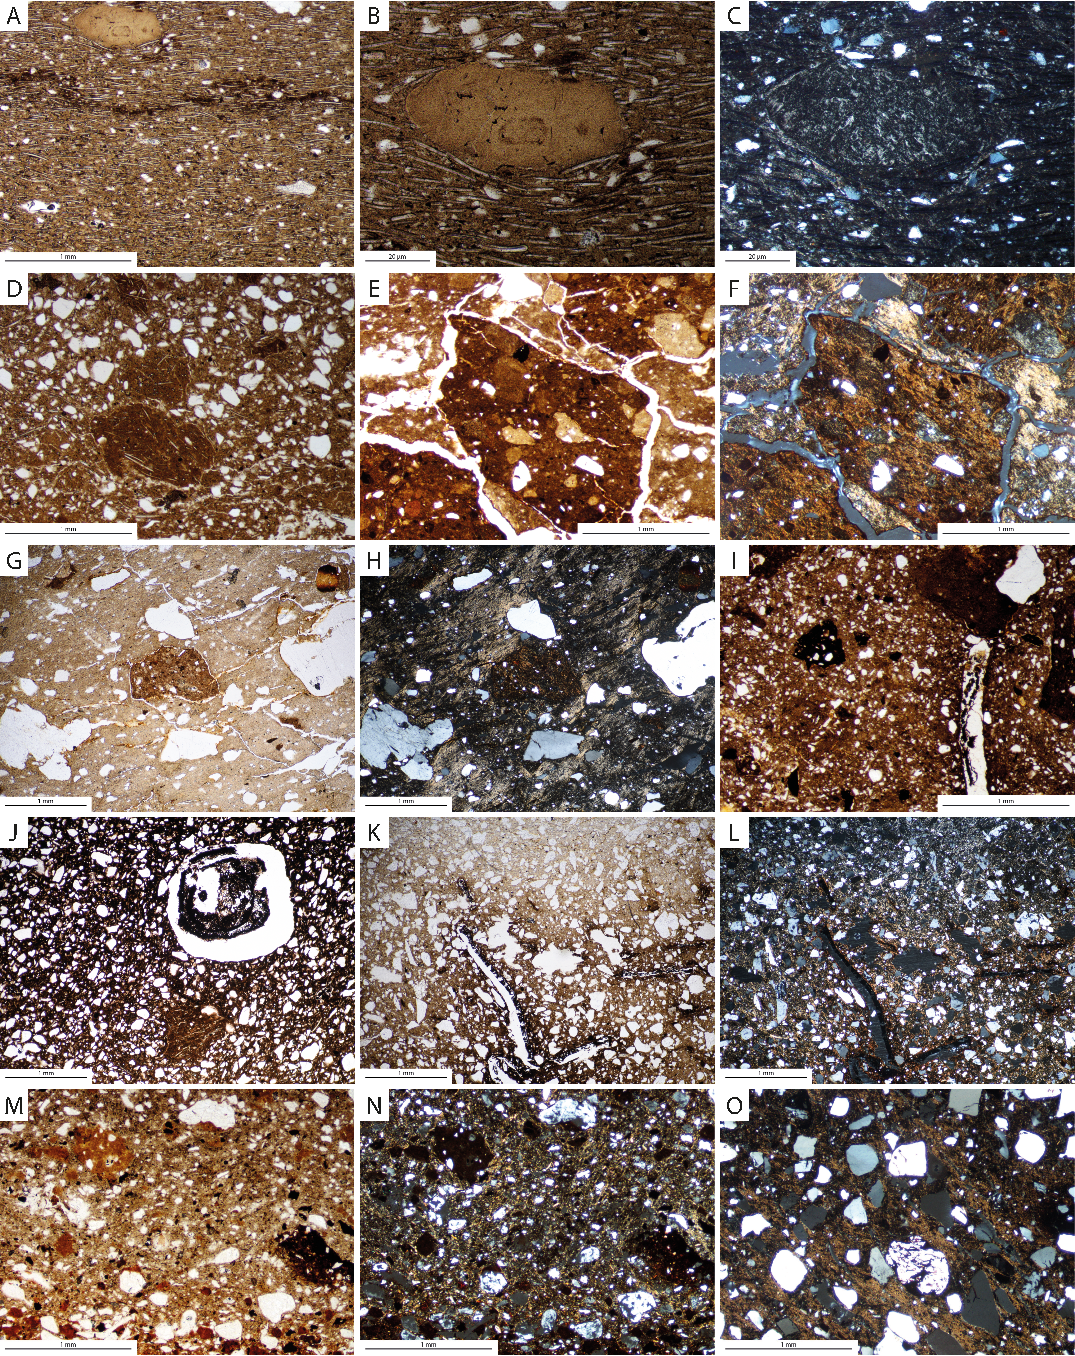
\includegraphics[width=\textwidth]{Fig_Thinsections.pdf}
	% A-C: PIK 87/1-2:70 #55 = sponge spicules rich river clays @PIK
	% D: MON 83/101:3 #51 = grog temper
	% E-F: SNP 03-4:5 #46 = grog temper
	% G-H: SNP 03-4:1 #42 = grog temper cf Fig. SNP pottery #1
	% I: SNP 03-7:1 #44 = gras temper cf Fig. SNP pottery #6
	% J: MON 83/101:4 #52 = grog & seed (org) temper
	% K-L: WAF 83/16-2:3 #48 = gras temper
	% M-N: PIK 87/1-1:35 #11 = terrestrial clays
	% O: PIK 87/501:4 #57 = terrestrial clays
	\caption{Photomicrographs of ceramic thin-sections from Pikunda (A--C, M--O), Monkoto (D,J), SNP-03 (E--I), and Wafanya (K--L) in plain-polarized light (PPL; A--B, D--E, G, I--K, M) and cross-polarized light (XPL; C, F, H, L, N--O). Basal petro-fabrics can be devided based on usage of river clays rich in sponge spicules (A--C), tempering with grog (D--H), tempering with grog and charred plant matter (I--J), tempering with charred plant matter (K--L), and usage of clays with the coarse fraction consisting solely of minerals (M--O).}
	\label{fig:thinsections}
\end{figure*}

\subsection{Petrography}

The petrographic analysis of 40 sherds points at similarities and difference that can best be collated in three main petro-fabrics. The qualitative classification is supported by the results of the multivariate correspondence analysis (MCA) of the nominal categorical data derived of the documented features \citet[1336-1137 Appendix 2--3]{Cau.2004}. The main distinction observed during the petrographic analysis concerns the presence or absence of sponge spicules as dominating component of the coarse fraction (Fig.~\ref{fig:thinsections}A--C). Sponge spicules appear as elongated isotropic rods in plane-polarized light (PPL, Fig.~\ref{fig:thinsections}A--B) and are the remains of the micro-sized, siliceous skeletons of freshwater sponges. Samples rich in sponge spicules also regularly show no or only little birefringence, resulting in a undifferentiated or slightly stipple-speckled b-fabric of the fine fraction. Samples rich in sponge spicules were grouped into petro-clusters 1--2 in the samples from case study I (Fig.~S2a) and cluster 3--5 in the samples from the Luilaka (Fig.~S2b). 

Out of the 28 samples from the western Congo Basin, 18 are grouped into petro-cluster 2 and represent the 'typical' sponge spicules rich petro-fabric 1 (Fig.~\ref{fig:synthesis}). The presence of sponge spicules is a distinct indicator for the source clay originating from a fluvial source, very similar to the main potters village of Ikenge on the Ruki river \citep{Eggert.1980c}. Clay briquettes and samples from vessels produced at this village, which are not included into this study, unanimously show high presence of sponge spicules. The samples occasionally also contain indicators for clay mixing. The second most prominent constituent of the coarse fraction of these samples is sub-angular quartz in a unimodal grain-size distribution. Among the rarer components of the coarse fraction are muscovite and occasionally biotite, tourmaline, staurolite, kyanite, and zircon. Petro-cluster 1 from the western Congo Basin (Fig.~S2a), despite also showing high concentrations of sponge spicules, is set apart from the main petro-cluster 2 due to samples showing unistriated b-fabrics of the fine fraction and considerably lesser quantities of quartz in the coarse fraction. This cluster is comprised of one sample from Pikunda and three samples from Munda (Fig.~S14, S27, S28, S39). Together, petro-clusters 1 and 2 from the western Congo Basin (Fig.~S2a) only contain samples pertaining to the Early Iron Age styles Pikunda-Munda, a single sherd pertaining to the Lusako style \citep[Fig.~S21;][104--107]{Wotzka.1995}, and the Late Iron Age Ebambe style. Out of the 22 sherds in petro-clusters 1 and 2 from the western Congo Basin (Fig.~S2a), only two sherds show no signs of sponge spicules (Fig.~S17, S18). 

Among the samples from the Luilaka, six out of the 12 samples showed differing proportions of sponge spicules. They are represented by petro-clusters 3--5 from the dataset from the Luilaka (Fig.~S2b). These are the single sample from SNP-01 (Fig.~S45) and two sherds from Wafanya (Fig.~S41, S44). The three samples from Monkoto only contained smaller amounts of sponge spicules (Fig.~S50, S51, S52). Two of these (Fig.~S50, S51) show an undifferentiated b-fabric of the fine fraction, while the others show unistriation of the birefringence of the fine fraction. Two of the samples from Monkoto that showed small amounts of sponge spicules (Fig.~S51, S52) also contain grog and organic matter. They are thus grouped into petro-fabric 3 (Fig.~\ref{fig:synthesis}).

The second basal petro-fabric describes samples that show no signs of sponge spicules, but a coarse fraction consisting mainly of mineral components (Fig.~\ref{fig:thinsections}M--O). This petro-fabric is best represented by petro-cluster 3--4 from the western Congo Basin (Fig.~S2a), which only contains sherds of the Late Iron Age Mandombe style (Fig.~S13, S15) as well as three modern samples from Pikunda (Fig.~S24, S25, S26) and one of the three Early Iron Age sherds associated with the Ngbanja style (Fig.~S20). Thus, petro-fabric 2 is only comprised of samples from the site of Pikunda and five out the six samples date in to the Late Iron Age. The fine fraction of these samples often shows considerable birefringence, often in a stipple-speckled b-fabric. Other than samples of petro-fabric 1, which usually shows no or very narrow voids, the sherds of petro-fabric 2 display voids, some in U-shaped (Fig.~S17, S26), diagonal (Fig.~S24, S25), or wall-parallel (Fig.~S20) configurations in relation to the plane of the section. The main component of the coarse fraction of these samples is sub-angular quartz, in either a unimodal (Fig.~S18, S24, S25) or bimodal grain-size distribution (Fig.~S13, S15, S17, S20, S26). The one sherd associated with the Early Iron Age Ngbanja style grouped in petro-fabric 2 shows not only a bimodal grain-size distribution of the quartz component, but the bigger grains also show particularly angular edges, indicative of part of the quartz in that sample originating from crushing of quartz for additional tempering of the clay. The other most prominent mineral constituents of the coarse fraction of samples grouped into petro-fabric 2 are fragments of sandstone (Fig.~S18, S20, S24, S26) and runiquartz (Fig.~S15, S20, S24, S25). Two samples contained very small fragments of plagioclase (Fig.~S13, S15). Besides that, the samples in this petro-fabric also contained muscovite, biotite, tourmaline, staurolite, and zircon. Non-mineral components of the coarse fractions of the samples in petro-fabric 2 are clay pellets (Fig.~ S13, S15, S20, S25) and charred organic matter (Fig.~S13, S15, S17). Noteworthy is a modern sherd that contained a slag fragment (Fig.~S24). A working hypothesis is that these clays, unlike the ones rich in sponge spicules (petro-fabric 1) were not necessarily sourced in the immediate proximity to the rivers. This hypothesis must remain untested until distinct clay samples from the region become available.

The third main petro-fabric is comprised of samples made from either clays that are very poor in sponge spicules or show no signs of sponge spicules altogether. The main characteristic of this petro-fabric is the presence of grog and/or plant matter (Fig.~\ref{fig:synthesis}), which are distinct temper agents known to be used through ethnographic reports \citep[33 Map 2]{Drost.1967}. This basal petro-fabric is further divided into three sub-fabrics: 3a are samples that contain grog as well as charred plant matter (Fig.~\ref{fig:thinsections}I--J, S49, S51, S52), 3b samples that contained grog but no charred plant matter (Fig.~\ref{fig:thinsections}D--H, S46, S47, S48), and 3c samples with charred plant matter and no grog (Fig.~S42, S43). As mentioned above, also three samples from the site of Pikunda in the western Congo Basin contain limited amounts of charred plant matter (Fig.~S13, S15, S17). But as indicated above, do to the distinct mineral components within the coarse fraction of these samples, they are better placed in basal petro-fabric 2. The petro-fabric 3b containing grog but no plant matter is represented by cluster 1 from the Luilaka (Fig.~S2b), while petro-fabric 3c containing charred plant matter and no grog is represented by cluster 2 (Fig.~S2b). All sherds in this main petro-fabric show a fine fraction with high birefringence, regularly in a stipple-speckled b-fabric, in one case with putative cross-striation (Fig.~S47). Similar to petro-fabric 2, the samples show wall-parallel (Fig.~S46, S48) or diagonal voids (Fig.~S49). Besides the mentioned grog and/or charred plant matter, the main constituent of petro-fabric 3 is sub-angular quartz in unimodal (Fig.~S43, S48) or bimodal grain-size distribution (Fig.~S42, S46, S47, S49). All samples contain muscovite, and some also contain tourmaline (Fig.~S42), staurolite (Fig.~S43), and zircon (Fig.~S43, S46). A noteworthy sample is a sherd from Monkoto (Fig.~S52) that shows tempering with plant matter, including seeds, as well as grog (Fig.~\ref{fig:thinsections}J). While the fine fraction of this samples clay matrix shows no sponge spicules, the grog particles were derived from pottery produced using fluvial clay rich in sponge spicules. 

\begin{figure*}[p]
	\begin{subfigure}[t]{\textwidth}
		\includegraphics[width=.98\textwidth]{Fig_XRF_pca_pik-mun.pdf}
		\vspace{1em}
		%\caption{Case study I: Western Congo Basin}
		\label{fig:xrf.pca.wCB}
	\end{subfigure}
	\begin{subfigure}[t]{\textwidth}
		\includegraphics[width=.98\textwidth]{Fig_XRF_pca_luilaka.pdf}
		%\caption{Case study II: Luilaka}
		\label{fig:xrf.pca.luilaka}
	\end{subfigure}
	\caption{Score and loading plots of PC 1 and 2 from the PCA's on the X-Ray intensities of six chemical elements from samples from the western Congo Basin (A--B, n = 31) and the Luilaka region (C--D, n = 12, Tab.~\ref{tab:samples}). Grey dots in A \& C show reference data derived from 169 samples from 59 sites in the Congo Basin that are not discussed in detail in this study. Colors correspond to Fig.~\ref{fig:chrono}.}
	\label{fig:xrf.pca}
\end{figure*}

\subsection{Geo-chemical characterization}

The chemical fingerprints of the studied samples show clear patterns that are described best per case study. The data from the western Congo Basin (Fig.~\ref{fig:xrf.pca}A--B) show a clear separation of two groups that can neither be traced back to the samples provenance nor dating exclusively. Samples from Pikunda (Fig.~S8) can be found in both groups, while all sherds from Munda (Fig.~S9) group together (Fig.~\ref{fig:xrf.pca}B), irrespective of them pertaining the to Early Iron Age Pikunda-Munda style or the modern Ebambe style (Fig.~\ref{fig:chrono}). This is seen as indication that all samples from Munda were produced using similar clays obtained in relative close proximity to each other, presumably close to the site. Thus, the studied pottery from Munda is viewed as local production. All sherds show, relatively to the other samples from the western Congo Basin, high amounts of silica (Si), titan (Ti) and aluminum (Al) (Fig.~\ref{fig:xrf.pca}B). Also in this group plot sherds from Pikunda pertaining to the Early Iron Age styles Pikunda-Munda and Lusako (Fig.~S7.1--5) as well as the Late Iron Age Ebambe pottery (Fig.~S7.12). The second group, showing distinctly higher concentrations of iron (Fe) and strontium (Sr) is comprised of samples associated with the Late Iron Age Ngoko pottery style tradition from Pikunda \citep[Fig.~S7.11--12;][]{Seidensticker.2021e,Seidensticker.2024} as well as three samples identified as stylistic outliers in the inventory of the Early Iron Age pit and described as part of the Ngbanja style \citep[Fig.~S7.6--8;][295--297]{Seidensticker.2021e}. Furthermore, this group also contains a sample from a vessel that was potted in 1987 at the site itself \citep[cf.][Fig.~15]{Seidensticker.2025}.

While sherds from Pikunda are present in both chemical groups and partially overlap with samples from Munda, the main differentiation is associated with the presence/absence of sponge spicules (Fig.~S5). All sherds pertaining to group 1, sensu samples representing the styles Pikunda-Munda and Ebambe, showed sponge spicules during the petrographic examination, while the samples in group 2 are void of spicules. The samples from the two sites only showed chemical differences in terms of their content of calcium (Ca) and trace elements that were removed due to a lack of specific calibration or potential post-depositional alterations such as rubidium (Rb), tantalum (Ta), and thorium (Th) (Fig.~S4). 

The chemical data from the Luilaka region (Fig.~\ref{fig:xrf.pca}C--D), while being more scattered than those from the western Congo Basin, show partial groupings of samples. Two sherds of the Bekongo style from Wafanya (Fig.~S12.5--6) as well as two sherds from the SNP-03 location (Fig.~S11.7) show similar chemical compositions characterized by higher amounts of iron (Fe) and silica (Si) (Fig.~\ref{fig:xrf.pca}D). Also chemically close are two sherds from the SNP-03 site (Fig.~S11.5) that are set apart from the other samples by their higher concentration in potassium (K) and aluminum (Al). The remainder of samples spread further across, generally showing increased amounts of strontium (Sr) and titanium (Ti). Notable is that the single sherd from SNP-01 that shows similarity of the Bokuma style (Fig.~S11.1) plots with samples from Wafanya and Monkoto (Fig.~S12.2--4, 7) and not the samples from SNP-03.

\begin{figure*}[!p]
	\begin{subfigure}[t]{.49\textwidth}
		\includegraphics[width=\textwidth]{Fig_microCT_Wotzka95_Tafel_69-5.jpg}
		\caption{}
		%\caption{Sampled vessel unit of the Bekongo style WAF 83/16-5:33 \citep[503 Pl. 69.5]{Wotzka.1995}.}
		\label{fig:waf83/16-3:33_drawing}
	\end{subfigure}\hspace{.5em}\hfill
	\begin{subfigure}[t]{.235\textwidth}
		\includegraphics[width=\textwidth]{Fig_microCT_IMG_20220809_084117.jpg}
		\caption{}
		%\caption{Photo of the sampled sherd.}
		\label{fig:waf83/16-3:33_photo}
	\end{subfigure}\hspace{.5em}\hfill
	\begin{subfigure}[t]{.235\textwidth}
		\includegraphics[width=\textwidth]{Fig_microCT_IMG_20211108_132303.jpg}
		\caption{}
		%\caption{Detail of the organic inclusion visible on the interior surface.}
		\label{fig:waf83/16-3:33_detail}
	\end{subfigure}\hfill
	\begin{subfigure}[t]{\textwidth}
		\includegraphics[width=\textwidth]{Fig_microCT_Screenshot_1.jpg}
		\caption{\vspace{1em}}
		%\caption{{\textmu}CT Scan at 35.5~{\textmu}m voxel size. Annotations indicate the locations of detailed images e--g. * indicates an additional seed only observed in this scan.}
		\label{fig:waf83/16-3:33_scan1}
	\end{subfigure}
	\begin{subfigure}[t]{.32\textwidth}
		\includegraphics[width=\textwidth]{Fig_microCT_organic-inclusion-xy.jpg}
		\caption{}
		%\caption{Virtual cross-section of the seed at 15~{\textmu}m voxel size.}
		\label{fig:waf83/16-3:33_scan3}
	\end{subfigure}\hspace{.5em}\hfill
	\begin{subfigure}[t]{.32\textwidth}
		\includegraphics[width=\textwidth]{Fig_microCT_organic-inclusion-volume-rendering-xz.jpg}
		\caption{}
		%\caption{Reconstructed lateral view of seed at 15~{\textmu}m voxel size.}
		\label{fig:waf83/16-3:33_scan2}
	\end{subfigure}\hspace{.5em}\hfill
	\begin{subfigure}[t]{.32\textwidth}
		\includegraphics[width=\textwidth]{Fig_microCT_Screenshot2.jpg}
		\caption{}
		%\caption{Potential grass temper at 35.5~{\textmu}m voxel size.}
		\label{fig:waf83/16-3:33_scan4}
	\end{subfigure}\hfill
	\caption{Sherd from Wafanya. (a) Sampled vessel unit of the Bekongo style WAF 83/16-5:33 \citep[503 Pl. 69.5]{Wotzka.1995}. (b) Photo of the sampled sherd. (c) Detail of the organic inclusion visible on the interior surface. (d) 3D volume render of the sampled sherd. (e) {\textmu}CT cross section of the seed. (f) 3D volume render of the seed, lateral view. (g) 3D volume render of potential grass temper.}
	\label{fig:waf83/16-3:33_microCT}
\end{figure*}

\subsection{Organic inclusions ({\textmu}CT Scan)}

The {\textmu}CT scans of a sherd pertaining to the Bekongo style (Fig.~\ref{fig:chrono}) from Wafanya (Fig.~S43) revealed multiple inclusions of potentially organic origin. The object of interest (Fig.~\ref{fig:waf83/16-3:33_scan1}*) has a double conical shape with a spiralling internal structure and is 2.4~mm long and 1.3~mm in diameter (Fig.~\ref{fig:waf83/16-3:33_scan3}--f). A thin-section from a sherd from Monkoto shows a similar feature (Fig.~S52a). The {\textmu}CT scan revealed another similar inclusion (Fig.~\ref{fig:waf83/16-3:33_scan1}**) and multiple planar voids with remnants of inclusions. The biggest of these elongated voids with potential remnants of an organic inclusion is about 9~mm long, 1.5--2~mm wide and around 0.2~mm thick (Fig.~\ref{fig:waf83/16-3:33_scan4}). It is interpreted as potential grass leaves \citep[Fig.~S42c--d;][]{Toth.2023}.

\begin{figure*}[!tb]
	\includegraphics[width=\textwidth]{Fig_Synthesis.pdf}
	\caption{Chrono-spatial overview of petro-fabrics identified at the studied sites. Colors correspond to Fig.~\ref{fig:chrono}.}
	\label{fig:synthesis}
\end{figure*}

\section{Discussion}

\subsection{Clay sourcing and preparation strategies}

The results from this study show patterns within the mineralogical and chemical makeup of the studied ceramics that point at distinct preferences concerning clay sourcing and preparation among potters' communities of practice in the western as well as Inner Congo Basin (Fig.~\ref{fig:synthesis}). The most distinct feature observed during the petrographic analysis is the presence/absence of the sponge spicules, which are regarded as clear identifier for the usage of fluvial clays. Examples for the usage of such clays are rare in the archaeological literature of sub-Saharan Africa. In the Americas, especially Amazonia, sponges known as "cauixi" are well known to have been used as temper agents in pre-Columbian pottery \citep{Linne.1932,Linne.1957,Cordell.1993,Costa.2004,Ottalagano.2016,Rodrigues.2017,Bloch.2019,LozadaMendieta.2019,Villagran.2022}. The usage of clay naturally rich in sponges or the deliberate addition of sponges as temper agents are known to increase the mechanical rigidity of the vessel after firing \citep{Natalio.2015}. With respect to ceramics from Africa, only very few examples are known from Mali \citep{Brissaud.1986,Mcintosh.1989,Nixon.2017}, Sudan \citep{Adamson.1987}, and the East African great lakes region \citep[185]{Ashley.2005}, while they are a complete novelty for Central Africa \citep{Seidensticker.2025}. While a species identification was hampered by the lack of observed gemmules in the thin sections some potential candidates could be derived from a synthesis of spongillofauna in Africa by \citet{Manconi.2009}. While \textit{Metania pottsi} is distributed widely in the study area, its spicules often show conules on the surface \citep[38--47]{Manconi.2009}. Otherwise, the species is best identified based on their gemmuloscleres, which are lacking in the archaeological samples. Other species with matching features are either not documented in the western Congo Basin, such as \textit{Eunapius nitens} \citep[149--151]{Manconi.2009}, which shows very similar spicules, or are poorly documented in general, such as \textit{Trochospongilla philottiana} \citep[198--199]{Manconi.2009}. Especially the lack of observed gemmuloscleres is regarded as indicator that the observed spicules are the result of natural accumulation processes in the source clays and not artificial tempering of the clays with spongillofauna. 

A clear correlation between a sherds style and presence or absence of sponge spicules can be observed in teh western Congo Basin (case study I). All 13 sherds of the Pikunda-Munda style and all six samples of the Ebambe style showed high abundances of sponge spicules, while all sherds from the Mandombe style as well as the modern samples show no spicules (Fig.~\ref{fig:synthesis}). This indicates that potters communities in the western Congo Basin, followed shared recipes concerning clay sourcing. During the Early Iron Age, potters producing Pikunda-Munda style pottery unanimously sourced fluvial clays, potentially in rivers or streams nearby their villages. Chemical differences between the samples from Pikunda and Munda were mostly observed among unreliable elements such as calcium (CA) and trace elements such as rubidium (Rb), tantalum (Ta), and thorium (Th) (Fig.~S4). This led to samples of a similar mineralogical composition pertaining to the styles Pikunda-Munda and Ebambe overlapping in the statistical analysis after rigorous selection of elements to include (Fig.~\ref{fig:xrf.pca}B). In consequence, the question if Pikunda-Munda and Ebambe pottery were produced locally or in a centralized fashion at a single site with subsequently distribution via trading must remain subject of future research. Three sherds of the Ngbanja style (Fig.~S7.6--8), found together with the Pikunda-Munda style pottery at Pikunda (Fig.~S7.1,3--4) and initially believed to be supra-regional contact finds \citep[296--297]{Seidensticker.2021e}, show distinctly similar chemical composition to the modern ceramics produced at the site in 1987 (Fig.~\ref{fig:xrf.pca}B). The potters' community producing the Late Iron Age Mandombe style pottery found at Pikunda, which shares no stylistic resemblance to any pottery found along the Sangha river before \citep{Seidensticker.2025}, approached distinctly different clays that show no features clearly indicative of a fluvial origin. The lack of local clay samples impedes any progress toward popper provenancing of the pottery.

Thus, for the samples from the western Congo Basin one could conclude the following: at Munda, all samples, irrespective of their chronological phase, were produced using similar fluvial clays rich in sponge spicules (Fig.~\ref{fig:synthesis}), potentially even originating from the same source area. The Pikunda-Munda style pottery from Pikunda was produced using clays from a distinctly similar setting. This is particular interesting as the stylistic heritage of the potters producing the Pikunda-Munda style vanish in the 5th--6th century CE \citep{Seidensticker.2025}. During the Late Iron Age, potters producing Mandombe style pottery relied on different types of clays void of sponge spicules that are more similar to the clays used by modern potters (Fig.~\ref{fig:synthesis}). This general pattern shows how much the early stages of the \textit{chaîne opératoire} of potters during the Late Iron Age were differing from those followed by earlier communities. A similar finding was observed in the primary and secondary shaping phases \citep{Seidensticker.2025} and together these differences in the \textit{chaînes opératoires} point at a potential disruption of knowledge transfer during the setback in human activity between the 6th--10th century CE \citep{Seidensticker.2021}.

Along the Luilaka (case study II), the results indicate a very different history of approaches concerning clay sourcing and especially during clay preparation (Fig.~\ref{fig:synthesis}). The two samples of the Early Iron Age Monkoto style show a similar chemical composition (Fig.~\ref{fig:xrf.pca}D) and the presence of sponge spicules, although to a lesser extend compared to contemporaneous samples from the western Congo Basin, point at a fluvial clay source. While two samples (Fig.~S41, S50) showed no signs of artificial tempering, the second sample contained considerable amounts of grog and charred plant matter (Fig.~S51). This points at different clay preparation strategies, while relying on similar clay sources, among potters' producing this type of pottery. This distinct difference in the \textit{chaîne opératoire} within the Monkoto style can be viewed as potential sign that multiple communities produced the ceramics of this style. Also relying on fluvial clays rich in sponge spicules were the potters that produced the vessel unit found in SNP-01 (Fig.~S45), pertaining to the younger Bokuma style, as well as the Late Iron Age Longa sherd found at Wafanya (Fig.~S44). The samples of the styles Monkoto and Longa as well as the Bokuma style vessel unit found at SNP-01 have a strikingly similar chemical fingerprint (Fig.~\ref{fig:xrf.pca}D), indicating a potentially common origin. Noteworthy is that the potters producing the in-between dating Bekongo style (Fig.~\ref{fig:synthesis}) followed a distinctly different approach. Both samples show them being made using a clay void of sponge spicules and artificial tempering with organic matter, potentially leaves (Fig.~S42, S43). Based on the chemical data, the sherds found in SNP-03 might originate from a clay source potentially close-by the one used by the potters of the Bekongo style sherds from Wafanya (Fig.~\ref{fig:xrf.pca}D). In terms of their clay preparation, these samples shows consistent tempering using grog and in one case also plant matter. In summary, this indicated the presence of multiple contemporaneous potters' communities along the Luilaka river that use either fluvial clays rich in sponge spicules or temper their clays, which lack sponge spicules, with mixtures of grog and plant matter. The 8th--10th century CE seems to be a time of change in this pattern as all samples dating to this time-frame relied on clays void of sponge spicules and showed tempering with either grog and/or plant matter (Tab.~\ref{fig:synthesis}). Overall, the findings from these two case studies underline the notion of potters' preferences for clay sources being driven rather by customs than considerations towards the features of the resulting product  \citep{Day.2004}.

\subsection{Biased surveying along rivers}

The approach of the \textit{River Reconnaissance Project} of focusing on surveys along the rivers of the Congo Basin has been critiqued by \citet[34--36]{Bower.1986}, whose main point concerned the selection of sites for excavation being "more or less intuitive" and opportunistic and thus potentially biased \citep[13 Fnt.~9]{Seidensticker.2021e}. \citep[36]{Bower.1986} also remarked the inconclusive chronology discussed by \citet{Eggert.1983,Eggert.1984a} and linked those to the selection of locations for excavations solely in modern villages, which yield higher potentials for post-depositional disturbances. The main source for these issues were discrepancies between the stratigraphic results and radiocarbon datings. \citet[132--133]{Eggert.1987a} suspected that the cause for this might be systematic issues with the radiocarbon dating laboratory, that were revealed later \citep{Geyh.1990}. The detailed analysis of the inventories by \citet{Wotzka.1995} further resolved all prior issues with the chronology. While \citet[296]{Eggert.1993} agreed with \citet{Bower.1986} that the surveys are severely biased, the chosen approach enable the exploration of a vast area that was a near complete archaeological \textit{terra incognita} before. To estimate the effect of this bias, \citet[303--304]{Eggert.1983} conducted an inland-survey between Imbonga on the Momboyo river and Nkuse and Isaka-Elinga on the Salonga and Lotoko on the Busira river in 1983 \citep[Fig.~\ref{fig:map};][18 Ftn.~3, 26]{Wotzka.1995}. As this survey only yielded pottery types that were already known from surveys and excavations along the rivers the bias introduced by focusing on the rivers were deemed neglectable. 

The novel finds obtained from the Salonga National Park (SNP) are reason enough to revisit the hypothesis that river-centered surveys in the Congo Basin yield a reasonably good-enough sample of the regional development of pottery producing communities. Our novel finds do not only show distinct approaches in terms of clay sourcing, using clay void of sponge spicules, and preparation, extensive tempering using grog and plant matter, but also no robust stylistic connection to neighboring sites (Fig.~S11, S12). These novel finds, which do not constitute a 'missing link' between earlier and later types like the Entebbe pottery in the Great Lakes region of East Africa \citep{Ashley.2010,Reid.2013}, shed some first light on the variability of potters' communities living off the major rivers, a thus far desideratum. In contrast to our new findings, pottery obtained by \citet[113--114 Fig.~42]{Gillet.2013} around 10--30~km inland of the upper Sangha river in the western Congo Basin revealed only types known from the survey along the Sangha river \citep{Seidensticker.2021e}. While this equally singular observation does not hold any reliable informative value for the Luilaka area, it should be seen as indicator against generalizations. Consequently, further fieldwork is not only much needed, but should also include the regions inland of and between the major rivers. It must thus remain the subject of future research to determine the extent to which the river-bound surveys of the \textit{River Reconnaissance Project} introduced biases to the present analyses \citep{Wotzka.1995,Seidensticker.2021e}.

\subsection{Chronology of the Bekongo pottery style}

Lacking radiocarbon dates associated with the Bekongo style, \citet[162]{Wotzka.1995} reasons for a chronological position within the overlapping period of the styles Longa and Bondongo, but without a complete congruence with neither one style, based on stylistic reasoning. Addressing the challenging dating of the Longa pottery and the fact that the Bekongo pottery gets succeeded by the Wafanya pottery, \citet[198]{Seidensticker.2021e} proposed a provisional date between the 11th to 12th century CE for the Bekongo style. A newly obtained AMS date (Tab.~S1b: RICH-33240) for a carbonized seed retrieved from a potsherd pertaining to the Bekongo style (Fig.~\ref{fig:waf83/16-3:33_microCT}) offers, for the first time, a direct date for the Bekongo style. A {\textmu}CT-Scan offered a powerful non-destructive way to visualize and examine the sherd and its inclusions in 3D prior to extraction for dating (Fig.~\ref{fig:waf83/16-3:33_microCT}). The technique offers an effective means to preserve valuable artifacts, allowing destructive methods to be applied afterwards if necessary. The newly obtained radiocarbon date covers the late 9th to 10th century CE, thus shifting the former assessment by about two centuries. In consequence, the novel date indicates that the Bekongo pottery might be predating the Bondongo style, which is dated robustly into the 11th to 14th century CE \citep[138 Tab.~58]{Wotzka.1995}. It also predates a recently obtained AMS date for the Ngombe styles which shows very strong stylistic resemblances with the Longa pottery, found along the lower Sangha river \citep[12th to 13th c. CE; RICH-30867 in][Tab.~2]{Seidensticker.2024}. Accepting this date for the Ngombe pottery and the youngest of the available dates for the Longa style, dating into the 12th to 13th c. CE as well \citep[Hv-11572 in][127 Tab. 53]{Wotzka.1995}, would mean that the Bekongo style also predates the Longa pottery as well as all other pottery styles associated with the Bondongo style horizon \citep[224--225]{Wotzka.1995}.

Notably, the main assemblage from SNP-03 was radiocarbon dated into the late 8th to mid 10th century CE as well (Fig.~S1; Tab.~S1b: RICH-25317), a period which had been regarded as experiencing a potential supra-regional set-back in human activity \citep{Seidensticker.2021}. These two dates (Tab.~S1b: RICH-25317 \& RICH-33240), associated with distinct pottery inventories, thus might shed some light on the putative relic communities still present between the 6th to 10th century CE \citep[Fig.~S4]{Seidensticker.2021e}.

\section{Conclusions}

The main focal point of this paper is the reconstruction of clay sourcing and preparation strategies at two multi-phase sites in the western Congo Basin and three sites along the Luilaka river in the Inner Congo Basin. The results of the petrographic analysis of 40 and geo-chemical fingerprinting of 43 samples revealed distinct connections between stylistic classifications \cite{Wotzka.1995,Seidensticker.2021e} with clay sourcing and preparation strategies. The most prominent example for this is the unanimous reliance of un-tempered fluvial clays rich in sponge spicules by potters producing Pikunda-Munda style vessels in the western Congo Basin. The same pattern holds true for the younger Ebambe style pottery. Potters producing the younger Mandombe pottery on the other had unanimously relied on clay void of sponge spicules as did modern potters' at Pikunda, despite the fluvial sources certainly still being available. This shift in raw material sources reflects on the way in which potting is a learned behavior with knowledge being transferred from one generation to another in tight-nit social networks, often kinship.

A more dynamic situation was encountered at the sites along the Luilaka river. Here, communities producing similar looking pottery showed distinct differences in clay sources approached and clay preparation techniques in particular. Features such as grog and charred plant remains point at deliberate temping of source clays, a distinct behavior that is difficult to asses for mineralogical constituents of a sherds coarse fractions such as sponge spicules or mineral components. Based on the limited set of samples studied from this region the most prominent observation is a distinct change away from clearly untempered fluvial clays to clays that were systematically tempered with grog and/or plant matter during the 8th--10th century CE. A later sample indicates that these changes have not been permanent and that clay sourcing strategies returned to prior approaches.

Furthermore, our novel finds from the Salonga National Park (SNP) reported here shed light on the inherent bias of the existing chrono-stylistic frameworks developed for the region \citep{Wotzka.1995,Seidensticker.2021e} with the river-bound surveys potentially having missed essential products of pottery producing communities in the Congo Basin. Furthermore, two novel radiocarbon dates, one dating the main inventory found in the SNP-03 and a organic inclusion in a sherd from the nearby site of Wafanya coincide with a previously reported supra-regional setback in human activity in Central Africa \citep{Seidensticker.2021e}. These novel dates and pottery types, although very isolated, could, at least on a local scale, point at putative refuges of relic communities bridging the existing chronological gap.

\section{Acknowledgments}

Special thanks go to Manfred K. H. Eggert for granting access to the findings from his project and supporting all aspects of this research.

DS designed this research and wrote the manuscript. DS conducted mineralogical identification and elemental analysis with help of FM, who furthermore provided the pXRF equipment of the RMCA for the elemental analysis. WH contributed potsherds found during digging of pedo-anthra\-cological test pits in the Salonga National Park. GF conducted the {\textmu}CT scannin, with access being provided by VC.

DS was supported by a FWO postdoctoral scholarship (senior) 1287922N. Thanks goes to UGCT for usage of {\textmu}CT scanning equipment and the authors acknowledge the Ghent University Special Research Fund (BOF-UGent) for the support to UGent Core Facility UGCT (BOF.COR.2022.0009) and FWO grant S000619N.

Further thanks goes Elena Marinova-Wolff (University Tübingen) for help with extracting the charred plant matter in a potsherd from Wafanya.

All coauthors commented on and approved the manuscript.

\subsection{Data Availability}

All data and computer code generated during this research is available here: \url{https://github.com/dirkseidensticker/OnOffRivers}.

\bibliographystyle{elsarticle-num-names}
%\bibliographystyle{elsarticle-harv}
\bibliography{bib.bib}

\end{document}